\section{MUIFOLD}

MUIFOLD is a framework for building applications with interactions
between a large display and multiple concurrent mobile clients.
Before discussing the specifics of the architecture and
implementation, we first layout some overall design goals that
we had for our system.

\begin{enumerate}
    \item \textbf{Utilize web-based technologies.} As shown by
    the prior work, by exclusively using web-based technologies
    for the display and mobile clients, this greatly lowers the
    barrier of entry for users and as opposed to requiring custom
    native applications they must install. This also makes it easier
    to build new content given the overall ubiquity of the web.
    \item \textbf{Multi-User Support.} Our application should
    be able to support multiple mobile clients simultaneously.
    \item \textbf{Have low latency between interactions of client and display.} When a user performs some action on their client, the
    display server should reflect that change relatively quickly,
    aiming for under 70ms to prevent potential loss of precision
    in various tasks~\cite{ivkovic_quantifying_2015}.
    \item \textbf{Provide ability to handle generic web pages in
    addition to custom built pages.} In an ideal world, all
    content would be custom built for our framework, users may
    have existing web technology that they would like to use. We
    should provide a way to seamlessly, and without any changes from
    the third-party site developer, integrate that the site in a
    seamless fashion, even if with relatively basic interaction.
\end{enumerate}

\subsection{Architecture}

For explaining the MUIFOLD system, we focus on the interplay between
Reagent, the display-worker, MUIFOLD, and the application web-pages, as
shown in Figure~\ref{fig:cais_implementation}.
Communication between the these components are largely built on top of  WebSockets,
which provide a full-duplex
communication channel over a single TCP connection. We utilize the
JavaScript Object Notation (JSON) format to transmit runtime
information. While this causes a slight increase on amount of bytes
sent over the wire compared to custom formats prior worked used,
this did not cause a noticeable degradation on performance and
latency as number of users scaled. Additionally, it is expected
that for custom client UIs that get opened, a WebSocket will
get opened that connects the client to a remote server hosting
the page they are interacting with, allowing for more
in-depth interaction.

\begin{comment}
%%% ignored, subsumed by diagram shown in chapter 2
\begin{figure}
\centering
  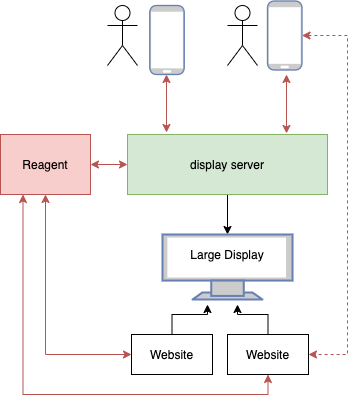
\includegraphics[width=0.8\columnwidth]{chapters/04_muifold/figures/muifold_architecture}
  \caption{Architecture of MUIFOLD. The red lines are WebSockets and the dotted line indicates an optional Web Socket depending on application needs.}
  \label{fig:architecture_muifold}
\end{figure}
\end{comment}

\subsection{Mobile Client}

The web-based mobile client, like other frameworks, is presented to the end-user through a simple webpage that the user opens on their
mobile device. This
can be either through scanning a QR code displayed on the large
display, or by manually typing in the URL. The client is
written using the React JS
framework~\footnote{https://reactjs.org/}, which provides a
high-level interface for building interactive UIs in JavaScript.
React provides a declarative language for the UI to be built in,
and helps to redraw the DOM as necessary as parts of the underlying
application state changes. Additionally, React allows us to define
the pieces of our UI as components, which makes it easy for us to
re-use pieces of the generic UI a user is greeted with when opening
the client in custom webview specific UIs as they need (e.g. like
for enabling pointing).
Out of the box, the mobile client presents the user with a generic
UI capable of interacting with any content displayed by the
large scale display, shown in Figure ~\ref{fig:mobile_start_ui}. The principle interaction methods in this
interface are pointing, left clicking, and scrolling content, similar
to the common mouse most users are familiar with from traditional
desktop and laptop computers.

\begin{figure}
\centering
  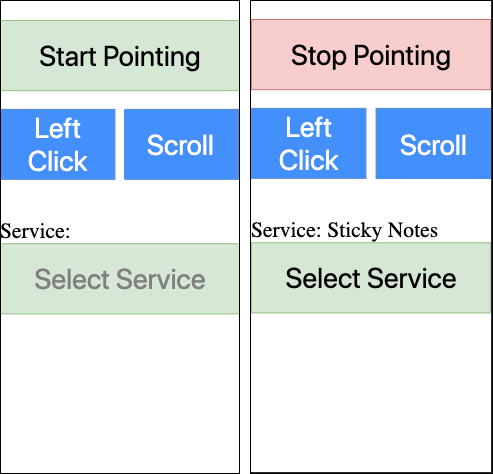
\includegraphics[width=0.65\columnwidth]{figures/generic_mobile_client}
  \caption{Generic interface for mobile client. Left view shows
  screen while not currently pointing. Right view shows client
  while actively pointing and cursor is over a display that has a custom application UI.}
  \label{fig:mobile_start_ui}
\end{figure}

Pointing is done through relative raycasting, relying solely
on the phone's builtin gyroscope and accelerometer and no additional
hardware through the DeviceOrientation API. When a user initially
connects, a
cursor is shown for the user at the center of the screen. Then,
while pointing is activated, for each tick the sensors report
their current degree, this is compared against the last measured
degree, taking the difference. This is then run through a smoothing
function~\cite{casiez_1_2012} to eliminate effects of natural
jitter, both in the sensors themselves and from slight hand
tremors. The client then reports this degree change to the display
server which translates this into a x,y pixel translation,
moving the cursor appropriately. The client then receives
information from the display server on if the cursor now is atop
a service that implements its own application specific UI. A
limitation of this approach is that over time, the cursor
eventually suffers from drift between where the user is pointing
to and where the cursor actually is. Self correction for this
though is easy enough by turning off pointing, re-adjusting
pointing position, and then turning back on pointing that it
this is not a great enough hindrance to ruin the approach. One thing
we did worry about was that as a user moved around the room and
interacted with the screen at different distances and angles, the
ratio of
degrees to pixels would need to change as well. In practice however,
we found that keeping this constant did not have any negative
effect on usage, so long as users stayed within 5-10 meters from
the ``sweet spot''.

Left clicking on the mobile interface is similar to how might
expect left-clicking with a standard mouse on a webview. Clicks that
happen within input fields, however will create a modal to appear
on the mobile interface that can be used to update that input
field, allowing the user to update the form in a mobile friendly
way. For example, clicking on a dropdown would show all of
the available options, clicking on an input would open the
keyborad, etc. Finally, when a user points at a webview that
is marked as having its own mobile UI, the button at the bottom
of the generic UI will activate with the name of the webview
appearing above it, such as in the right image in Figure
\ref{fig:mobile_start_ui}.

When opening a webview specific UI, the client gets the
URL for the webview's JavaScript to power its mobile UI. This
is then loaded dynamically, and injected into the running
application and run. It's expected that the JavaScript file will
either hook into the existing React root webview specific UIs or
can use vanilla JavaScript to build the DOM and manage it that way.
However, as stated above, with React, developers can utilize
components of the generic UI into their design as makes sense,
such as making available a button to toggle on / off pointing. The
only requirements for these UIs is that they must implement a button
that returns the user to the generic UI, and that they do not
overwrite the React root for the generic UI. Figure
\ref{fig:application_specific_ui} gives an example of how such
a UI might work for a specific application, in this case one
to create sticky notes. This UI re-uses the pointer component,
though shifted to the bottom of the screen, with custom content
for creating sticky notes. Hitting the ``Cancel'' button would
bring the user back to the generic UI.

\begin{figure}
\centering
  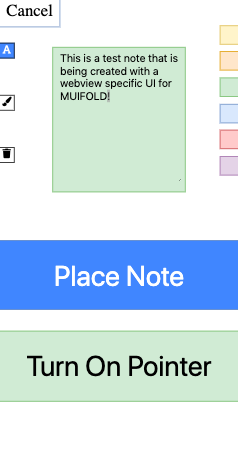
\includegraphics[width=0.40\columnwidth]{figures/application_specific_ui}
  \caption{Webview specific UI for a sticky notes application.}
  \label{fig:application_specific_ui}
\end{figure}
